\section{Methodology}
\label{sec:methodology}

Our system architecture (Fig.~\ref{fig:architecture}) processes trading days through a pipeline from data ingestion to LLM regime detection.

\begin{figure}[!htbp]
\centering
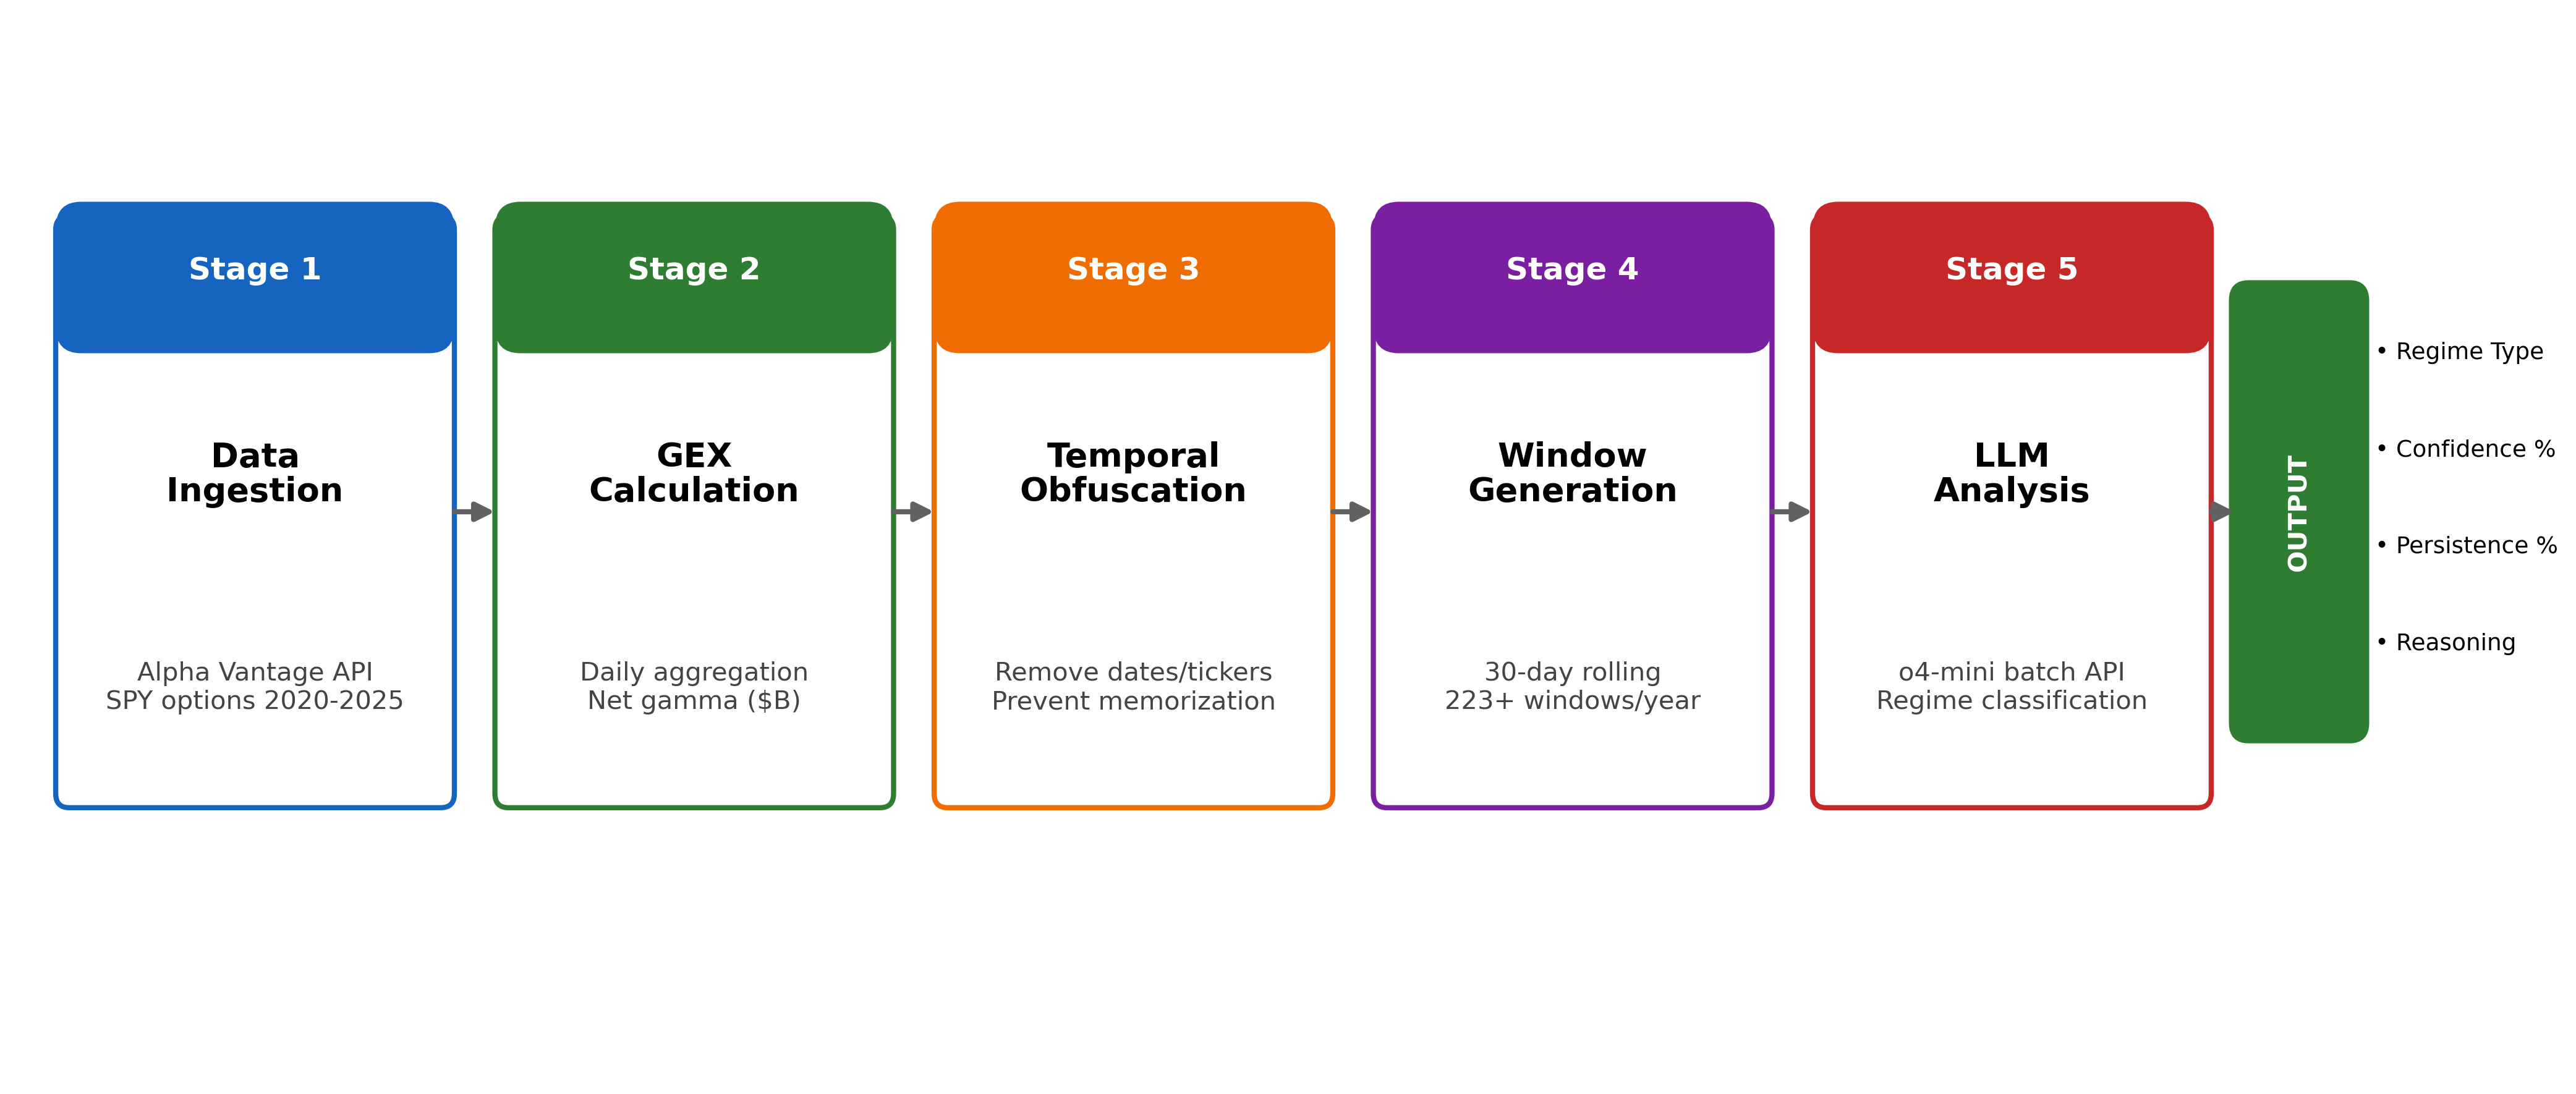
\includegraphics[width=\textwidth]{../figures/output/fig01_architecture.png}
\caption{System architecture. The pipeline processes trading days through five stages: data ingestion, GEX calculation, temporal obfuscation, 30-day window generation, and LLM analysis using OpenAI o4-mini via Batch API.}
\label{fig:architecture}
\end{figure}

\subsection{Regime Detection Framework}

Building on single-day obfuscation testing~\cite{regan2025obfuscation}, we extend the framework to detect \textit{persistent market regimes}---30-day windows exhibiting sustained dealer gamma positioning. We classify windows into four categories based on three structural metrics:

\textbf{Persistence}: Fraction of days sharing the dominant GEX sign ($P \geq 0.70$). \textbf{Magnitude}: Average absolute gamma exposure ($M \geq \$5\text{B}$). \textbf{Stability}: Sign flip count ($S \leq 5$).

Windows meeting all three criteria are classified as \textbf{persistent positive} or \textbf{persistent negative} regimes based on dominant sign. Windows failing persistence or stability are \textbf{transitional}; those meeting persistence/stability but not magnitude are \textbf{low conviction}. The 70\% persistence threshold ensures detected regimes exceed random binomial variation ($\approx 2.2\sigma$), while the \$5B magnitude threshold reflects economically significant dealer positioning.

\subsection{GEX Calculation}

Following standard market microstructure practice~\cite{anderegg2022impact,spotgamma2021}, we calculate dealer gamma exposure from end-of-day open interest:

\begin{equation}
\text{GEX} = \sum_i \pm \text{OI}_i \times \Gamma_i \times S^2 \times 0.01 \times 100,
\end{equation}

\noindent where $\Gamma_i$ is Black-Scholes gamma at strike $i$, $\text{OI}_i$ is open interest, $S^2$ scales gamma to dollar exposure, and call gamma enters positively while put gamma enters negatively. This open interest-based approach (GEX\_OI) measures dealer inventory positioning. Our 30-day temporal aggregation smooths daily measurement noise, and negative controls (Phase 2) validate framework robustness to measurement method.

\subsection{Temporal Obfuscation}

To prevent training data memorization, we apply obfuscation (Fig.~\ref{fig:obfuscation}): calendar dates become relative labels (``Day T-29'' through ``Day T+0''), ticker symbols become generic identifiers (``INDEX\_1''), and all event context is removed. The LLM receives only GEX magnitudes, spot prices, and days to expiration---forcing purely structural reasoning about dealer constraints.

\begin{figure}[!htbp]
\centering
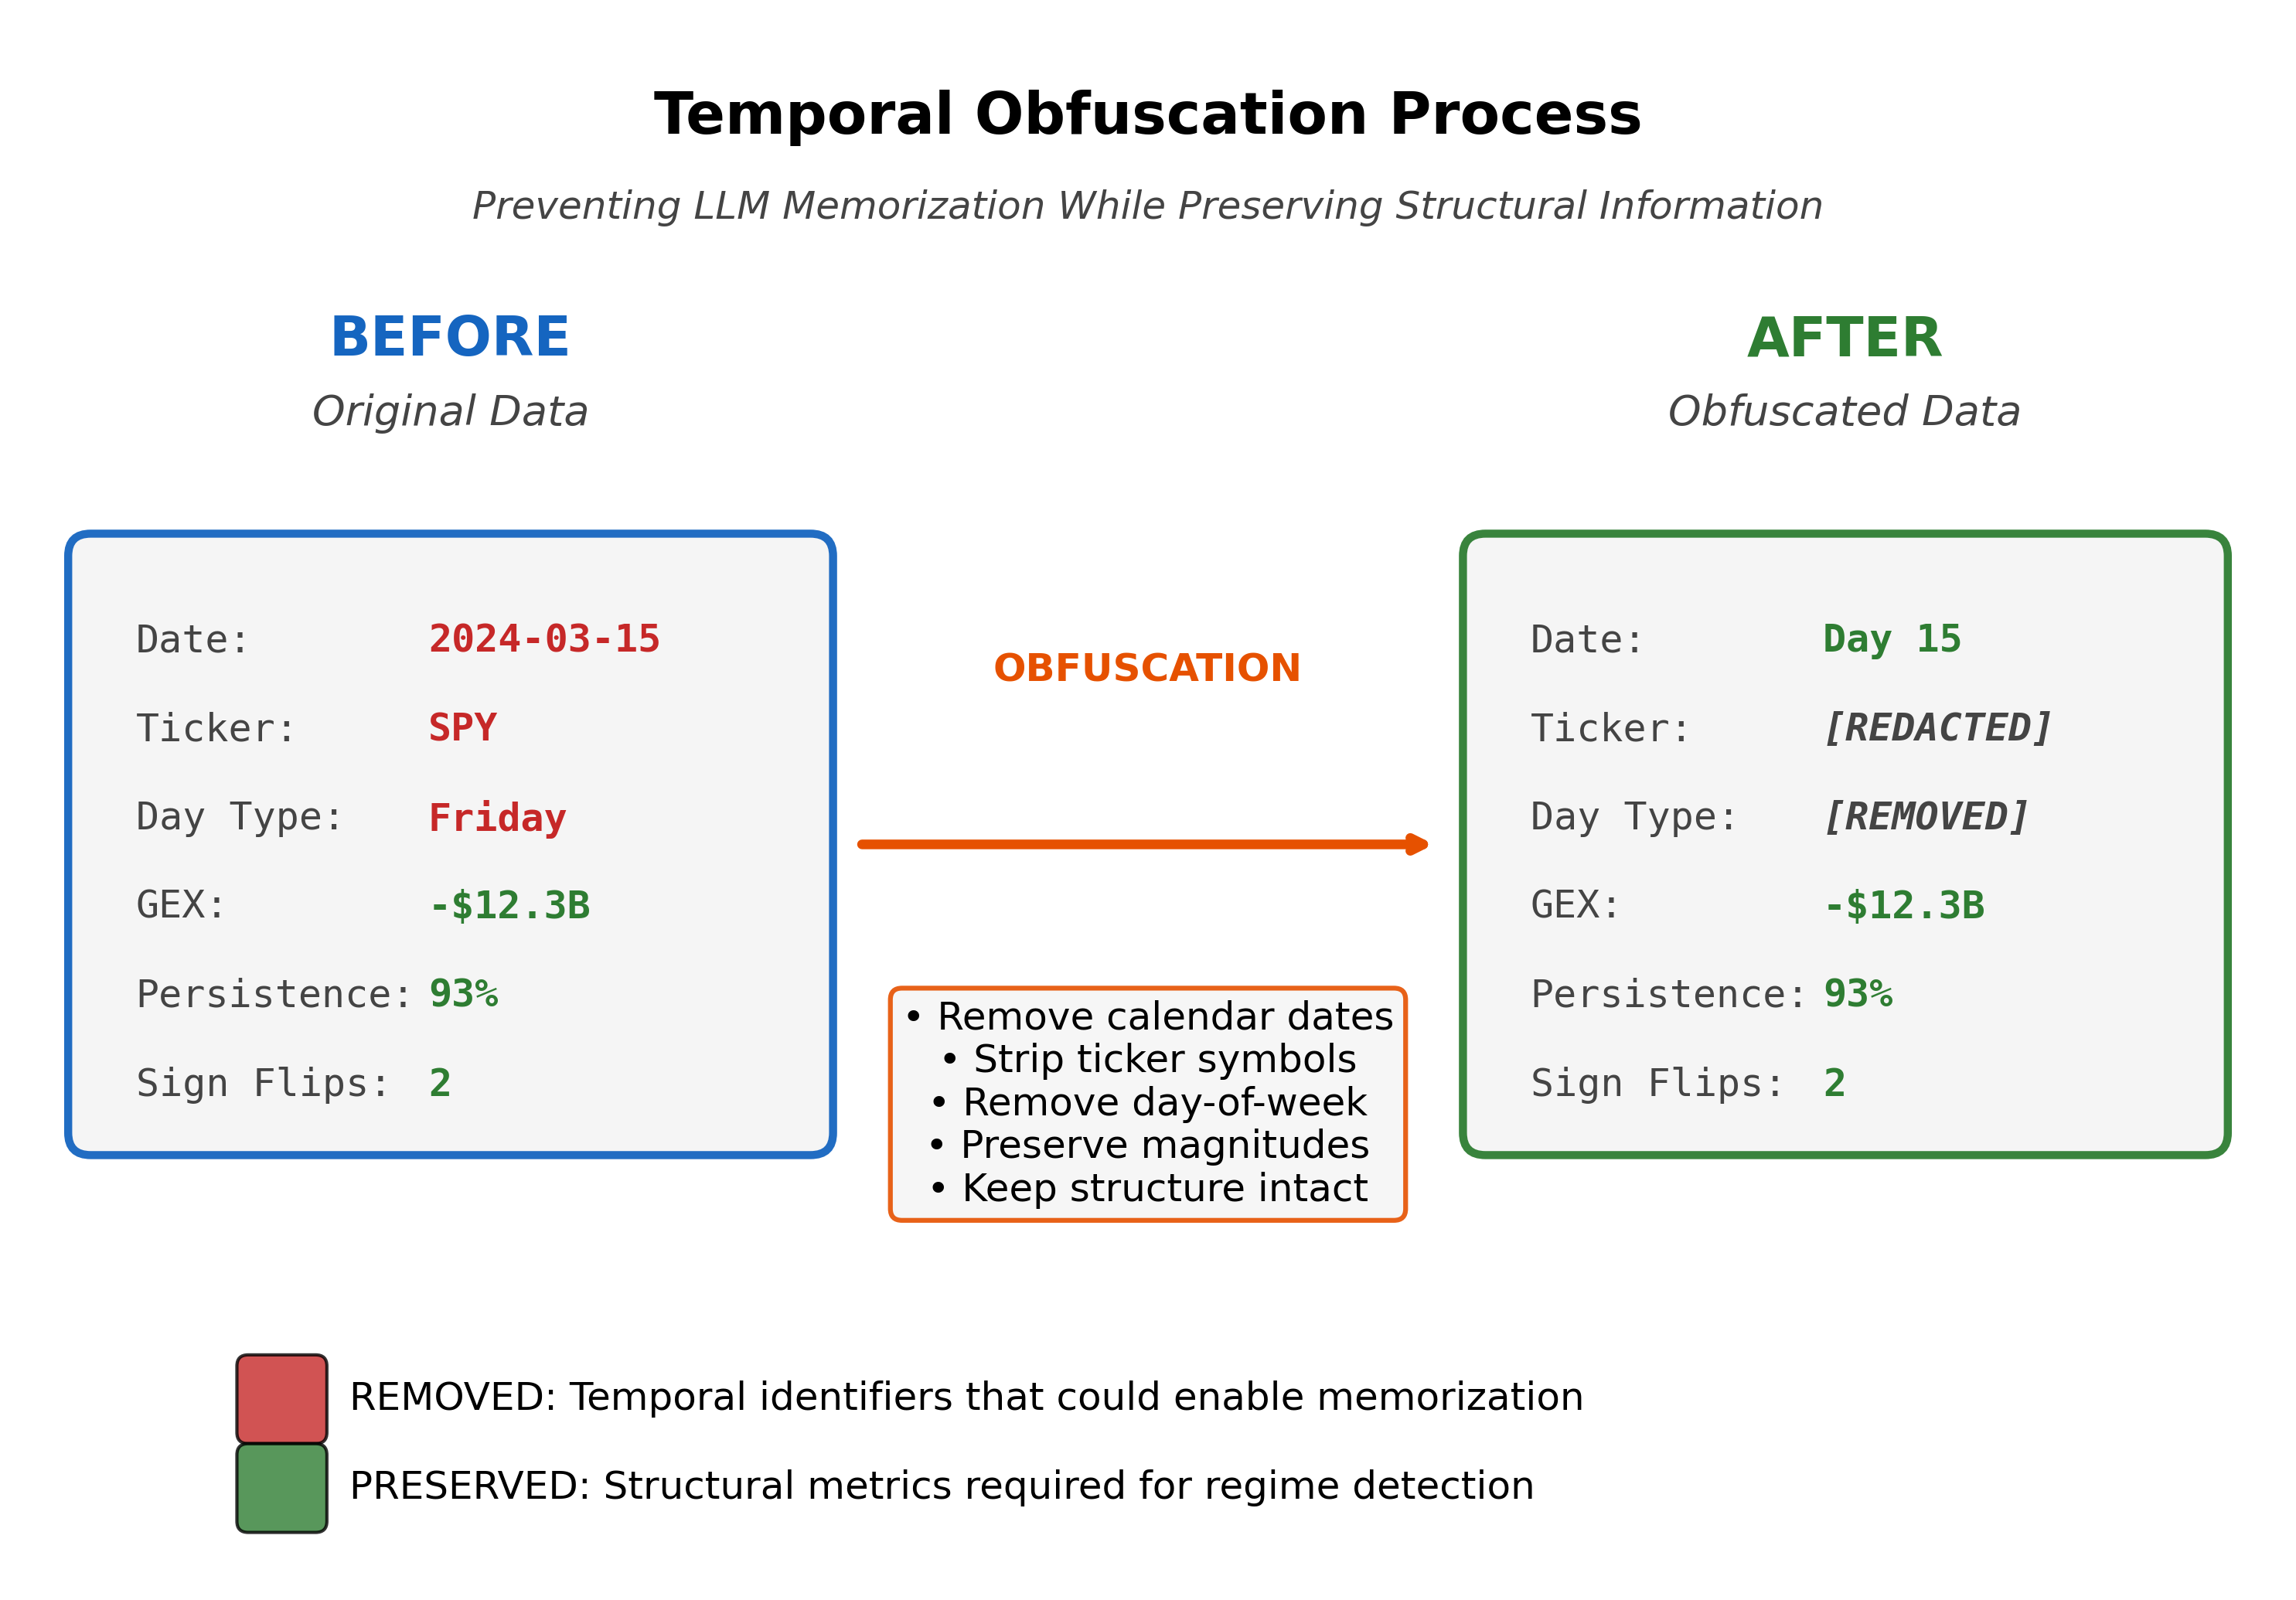
\includegraphics[width=0.95\textwidth]{../figures/output/fig03_obfuscation.png}
\caption{Temporal obfuscation process. Calendar dates, ticker symbols, and contextual markers are removed while preserving structural information.}
\label{fig:obfuscation}
\end{figure}

\subsection{Dataset and LLM Configuration}

\textbf{Data}: SPY (S\&P 500 ETF) options chains from Alpha Vantage Premium API. Primary dataset: 2024 (252 trading days, 223 rolling 30-day windows). Comparison dataset: 2020 (252 days, 223 windows). Multi-year extension: 2020--2025 (1,412 windows). Negative controls: 809 synthetic windows (shuffled, transitional, low-magnitude).

\textbf{LLM}: OpenAI o4-mini reasoning model~\cite{openai2024reasoning} with temperature=1.0, max tokens=16,384, processed via Batch API (asynchronous, 100\% completion rate). The model receives a system message (``financial market analyst identifying persistent dealer gamma regimes''), a 30-day obfuscated GEX sequence with classification criteria, and outputs structured JSON with regime type, confidence (0--100), reasoning trace, and computed metrics.

\subsection{Multi-Phase Validation}

We employ five validation phases spanning 2020--2025:

\textbf{Phase 1} (Q1 2024, 52 windows): Establish baseline detection rate. Success: 30--50\% detection demonstrating selectivity.

\textbf{Phase 2} (Negative Controls, 809 windows): Three synthetic tests---shuffle (404 windows, randomize day order), transitional (202 windows, 7--10 sign flips), low-magnitude (203 windows, scaled $<$\$5B). Expected: $<$20\% and $<$10\% false positive rates respectively.

\textbf{Phase 3} (Full 2024, 223 windows): Test generalization across all trading days.

\textbf{Phase 4} (2020 Comparison, 223 windows): Pre-0DTE baseline ($<$5\% 0DTE volume) versus post-0DTE (2024, $\approx$48\%).

\textbf{Phase 5} (2020--2025, 1,412 windows): Identify when structural shift occurred; test gradual versus sharp transition hypothesis.

For each LLM response, we extract stated metrics (persistence, magnitude, flips) and compare against ground truth. Windows with $>$5\% metric discrepancy are flagged for manual review.
